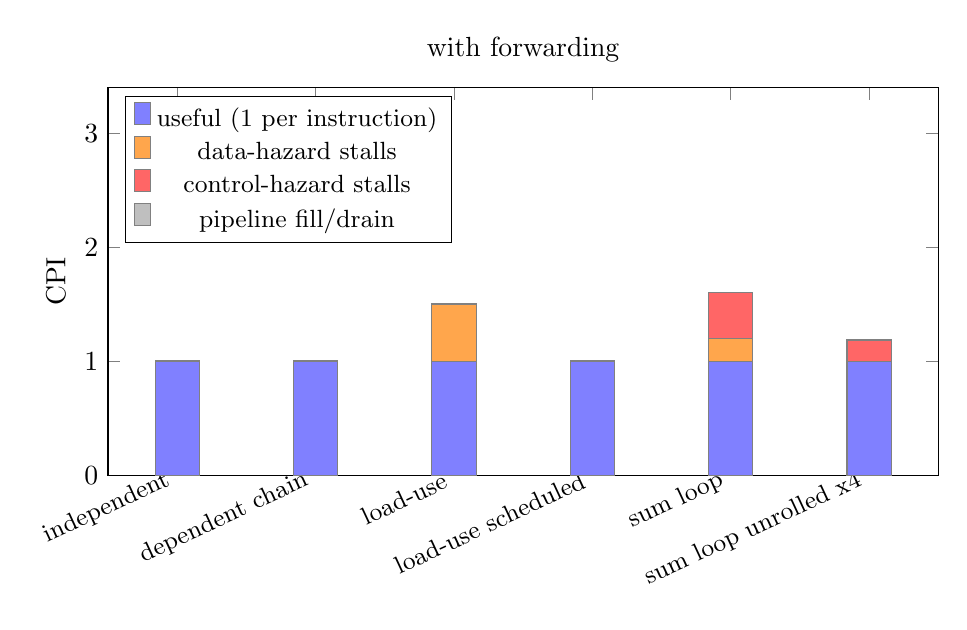
\begin{tikzpicture}
\begin{axis}[ybar stacked, width=\textwidth, height=6.5cm, bar width=16pt, ymin=0, ymax=3.4, ylabel={CPI}, title={with forwarding},
  symbolic x coords={independent,dependent chain,load-use,load-use scheduled,sum loop,sum loop unrolled x4}, xtick=data, x tick label style={rotate=25, anchor=east, font=\small},
  legend style={font=\small, at={(0.02,0.98)}, anchor=north west}, enlarge x limits=0.1]
\addplot+[fill=blue!50, draw=black!50] coordinates {(independent,1.000) (dependent chain,1.000) (load-use,1.000) (load-use scheduled,1.000) (sum loop,1.000) (sum loop unrolled x4,1.000) };
\addlegendentry{useful (1 per instruction)}
\addplot+[fill=orange!70, draw=black!50] coordinates {(independent,0.000) (dependent chain,0.000) (load-use,0.500) (load-use scheduled,0.000) (sum loop,0.200) (sum loop unrolled x4,0.000) };
\addlegendentry{data-hazard stalls}
\addplot+[fill=red!60, draw=black!50] coordinates {(independent,0.000) (dependent chain,0.000) (load-use,0.000) (load-use scheduled,0.000) (sum loop,0.400) (sum loop unrolled x4,0.182) };
\addlegendentry{control-hazard stalls}
\addplot+[fill=gray!50, draw=black!50] coordinates {(independent,0.004) (dependent chain,0.004) (load-use,0.004) (load-use scheduled,0.004) (sum loop,0.004) (sum loop unrolled x4,0.007) };
\addlegendentry{pipeline fill/drain}
\end{axis}
\end{tikzpicture}